\documentclass{standalone}
\usepackage{tikz}
\usetikzlibrary{patterns, positioning}

\begin{document}
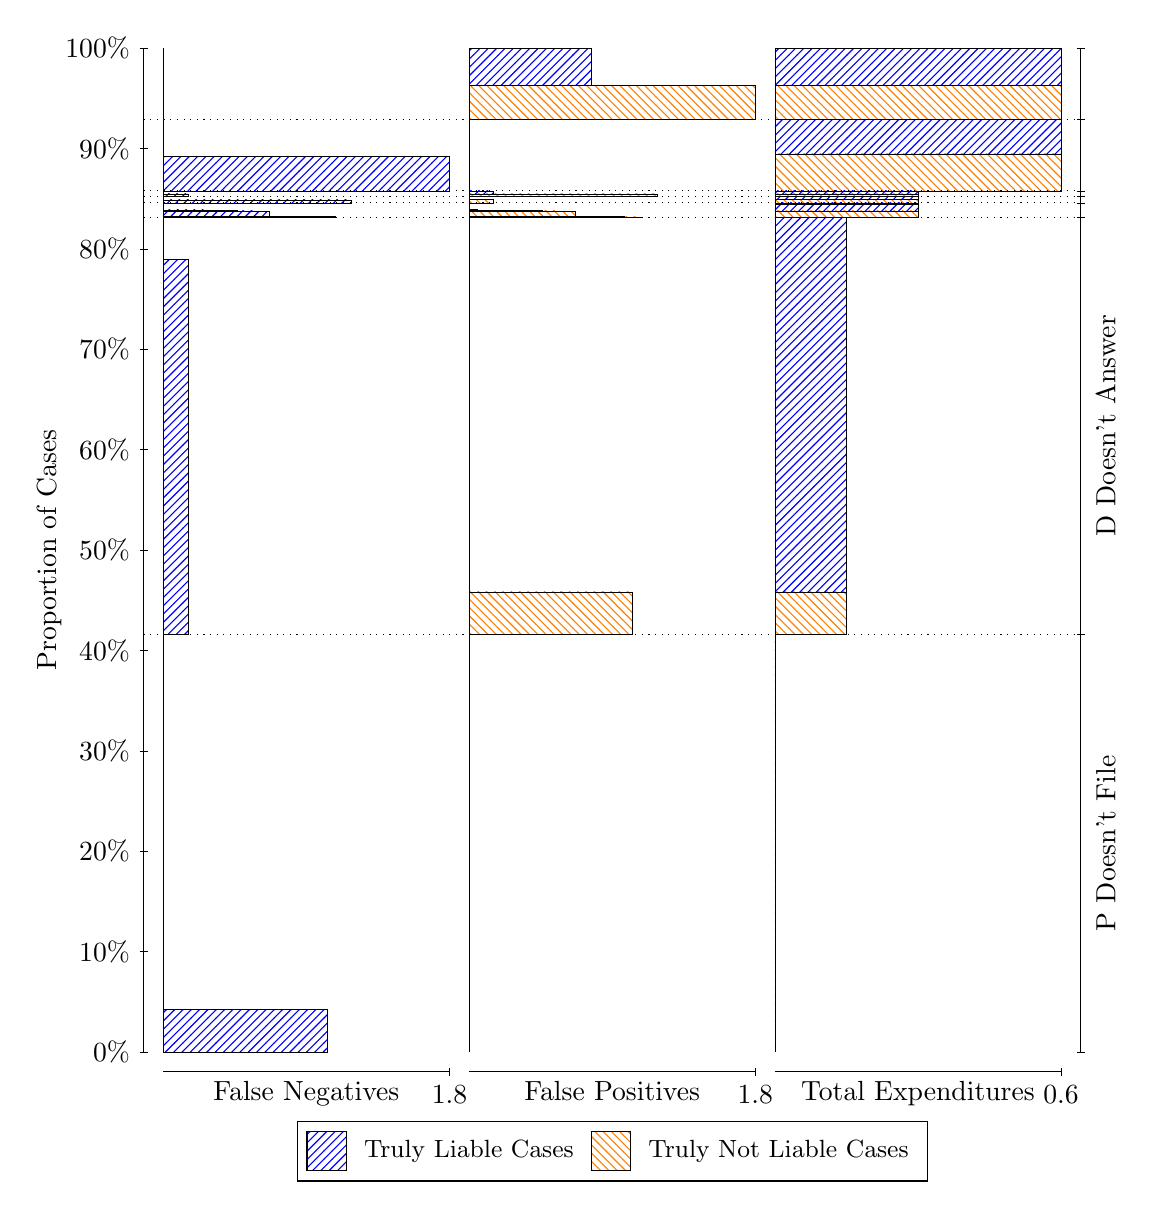
\begin{tikzpicture}
\draw[black, very thin] (1.5,1.75) -- (1.5,14.5);
\node[rotate=90, anchor=center] at (0.3, 8.125) {Proportion of Cases};
\draw[black, very thin] (1.45,1.75) -- (1.55,1.75);
\node[anchor=east] at (1.45, 1.75) {0\%};
\draw[black, very thin] (1.45,3.025) -- (1.55,3.025);
\node[anchor=east] at (1.45, 3.025) {10\%};
\draw[black, very thin] (1.45,4.3) -- (1.55,4.3);
\node[anchor=east] at (1.45, 4.3) {20\%};
\draw[black, very thin] (1.45,5.575) -- (1.55,5.575);
\node[anchor=east] at (1.45, 5.575) {30\%};
\draw[black, very thin] (1.45,6.85) -- (1.55,6.85);
\node[anchor=east] at (1.45, 6.85) {40\%};
\draw[black, very thin] (1.45,8.125) -- (1.55,8.125);
\node[anchor=east] at (1.45, 8.125) {50\%};
\draw[black, very thin] (1.45,9.4) -- (1.55,9.4);
\node[anchor=east] at (1.45, 9.4) {60\%};
\draw[black, very thin] (1.45,10.675) -- (1.55,10.675);
\node[anchor=east] at (1.45, 10.675) {70\%};
\draw[black, very thin] (1.45,11.95) -- (1.55,11.95);
\node[anchor=east] at (1.45, 11.95) {80\%};
\draw[black, very thin] (1.45,13.225) -- (1.55,13.225);
\node[anchor=east] at (1.45, 13.225) {90\%};
\draw[black, very thin] (1.45,14.5) -- (1.55,14.5);
\node[anchor=east] at (1.45, 14.5) {100\%};

\draw[black, very thin] (13.4,1.75) -- (13.4,14.5);
\draw[black, very thin] (13.35,1.75) -- (13.45,1.75);
\node[anchor=west] at (13.35, 1.75) {};
\draw[black, very thin] (13.35,7.0516) -- (13.45,7.0516);
\node[anchor=west] at (13.35, 7.0516) {};
\draw[black, very thin] (13.35,12.352) -- (13.45,12.352);
\node[anchor=west] at (13.35, 12.352) {};
\draw[black, very thin] (13.35,12.533) -- (13.45,12.533);
\node[anchor=west] at (13.35, 12.533) {};
\draw[black, very thin] (13.35,12.611) -- (13.45,12.611);
\node[anchor=west] at (13.35, 12.611) {};
\draw[black, very thin] (13.35,12.685) -- (13.45,12.685);
\node[anchor=west] at (13.35, 12.685) {};
\draw[black, very thin] (13.35,13.592) -- (13.45,13.592);
\node[anchor=west] at (13.35, 13.592) {};
\draw[black, very thin] (13.35,14.5) -- (13.45,14.5);
\node[anchor=west] at (13.35, 14.5) {};

\draw[black, very thin, pattern color=blue, pattern=north east lines] (1.75,1.75) rectangle (3.8262,2.2912);
\draw[black, very thin, pattern color=orange, pattern=north west lines] (1.75,2.2912) rectangle (1.75,7.0516);
\draw[black, very thin, pattern color=blue, pattern=north east lines] (1.75,7.0516) rectangle (2.0614,11.811);
\draw[black, very thin, pattern color=orange, pattern=north west lines] (1.75,11.811) rectangle (1.75,12.352);
\draw[black, very thin, pattern color=blue, pattern=north east lines] (1.75,12.352) rectangle (3.93,12.357);
\draw[black, very thin, pattern color=blue, pattern=north east lines] (1.75,12.357) rectangle (3.7224,12.359);
\draw[black, very thin, pattern color=blue, pattern=north east lines] (1.75,12.359) rectangle (3.5148,12.363);
\draw[black, very thin, pattern color=blue, pattern=north east lines] (1.75,12.363) rectangle (3.3071,12.365);
\draw[black, very thin, pattern color=blue, pattern=north east lines] (1.75,12.365) rectangle (3.0995,12.429);
\draw[black, very thin, pattern color=blue, pattern=north east lines] (1.75,12.429) rectangle (2.8919,12.431);
\draw[black, very thin, pattern color=blue, pattern=north east lines] (1.75,12.431) rectangle (2.6843,12.436);
\draw[black, very thin, pattern color=blue, pattern=north east lines] (1.75,12.436) rectangle (2.4767,12.439);
\draw[black, very thin, pattern color=blue, pattern=north east lines] (1.75,12.439) rectangle (2.269,12.443);
\draw[black, very thin, pattern color=orange, pattern=north west lines] (1.75,12.443) rectangle (1.75,12.533);
\draw[black, very thin, pattern color=blue, pattern=north east lines] (1.75,12.533) rectangle (4.1376,12.571);
\draw[black, very thin, pattern color=orange, pattern=north west lines] (1.75,12.571) rectangle (1.75,12.611);
\draw[black, very thin, pattern color=blue, pattern=north east lines] (1.75,12.611) rectangle (2.0614,12.649);
\draw[black, very thin, pattern color=orange, pattern=north west lines] (1.75,12.649) rectangle (1.75,12.685);
\draw[black, very thin, pattern color=blue, pattern=north east lines] (1.75,12.685) rectangle (5.3833,13.121);
\draw[black, very thin, pattern color=orange, pattern=north west lines] (1.75,13.121) rectangle (1.75,13.592);
\draw[black, very thin, pattern color=orange, pattern=north west lines] (1.75,13.592) rectangle (1.75,14.029);
\draw[black, very thin, pattern color=blue, pattern=north east lines] (1.75,14.029) rectangle (1.75,14.5);
\draw[black, very thin, pattern color=orange, pattern=north west lines] (5.6333,1.75) rectangle (5.6333,6.5104);
\draw[black, very thin, pattern color=blue, pattern=north east lines] (5.6333,6.5104) rectangle (5.6333,7.0516);
\draw[black, very thin, pattern color=orange, pattern=north west lines] (5.6333,7.0516) rectangle (7.7095,7.5922);
\draw[black, very thin, pattern color=blue, pattern=north east lines] (5.6333,7.5922) rectangle (5.6333,12.352);
\draw[black, very thin, pattern color=orange, pattern=north west lines] (5.6333,12.352) rectangle (7.8133,12.356);
\draw[black, very thin, pattern color=orange, pattern=north west lines] (5.6333,12.356) rectangle (7.6057,12.358);
\draw[black, very thin, pattern color=orange, pattern=north west lines] (5.6333,12.358) rectangle (7.3981,12.363);
\draw[black, very thin, pattern color=orange, pattern=north west lines] (5.6333,12.363) rectangle (7.1905,12.365);
\draw[black, very thin, pattern color=orange, pattern=north west lines] (5.6333,12.365) rectangle (6.9829,12.43);
\draw[black, very thin, pattern color=orange, pattern=north west lines] (5.6333,12.43) rectangle (6.7752,12.431);
\draw[black, very thin, pattern color=orange, pattern=north west lines] (5.6333,12.431) rectangle (6.7752,12.431);
\draw[black, very thin, pattern color=orange, pattern=north west lines] (5.6333,12.431) rectangle (6.5676,12.435);
\draw[black, very thin, pattern color=orange, pattern=north west lines] (5.6333,12.435) rectangle (6.36,12.438);
\draw[black, very thin, pattern color=orange, pattern=north west lines] (5.6333,12.438) rectangle (6.1524,12.442);
\draw[black, very thin, pattern color=blue, pattern=north east lines] (5.6333,12.442) rectangle (5.7371,12.446);
\draw[black, very thin, pattern color=blue, pattern=north east lines] (5.6333,12.446) rectangle (5.6333,12.533);
\draw[black, very thin, pattern color=orange, pattern=north west lines] (5.6333,12.533) rectangle (5.9448,12.573);
\draw[black, very thin, pattern color=blue, pattern=north east lines] (5.6333,12.573) rectangle (5.6333,12.611);
\draw[black, very thin, pattern color=orange, pattern=north west lines] (5.6333,12.611) rectangle (8.021,12.647);
\draw[black, very thin, pattern color=blue, pattern=north east lines] (5.6333,12.647) rectangle (5.9448,12.685);
\draw[black, very thin, pattern color=orange, pattern=north west lines] (5.6333,12.685) rectangle (5.6333,13.156);
\draw[black, very thin, pattern color=blue, pattern=north east lines] (5.6333,13.156) rectangle (5.6333,13.592);
\draw[black, very thin, pattern color=orange, pattern=north west lines] (5.6333,13.592) rectangle (9.2667,14.029);
\draw[black, very thin, pattern color=blue, pattern=north east lines] (5.6333,14.029) rectangle (7.1905,14.5);
\draw[black, very thin, pattern color=orange, pattern=north west lines] (9.5167,1.75) rectangle (9.5167,6.5104);
\draw[black, very thin, pattern color=blue, pattern=north east lines] (9.5167,6.5104) rectangle (9.5167,7.0516);
\draw[black, very thin, pattern color=orange, pattern=north west lines] (9.5167,7.0516) rectangle (10.425,7.5922);
\draw[black, very thin, pattern color=blue, pattern=north east lines] (9.5167,7.5922) rectangle (10.425,12.352);
\draw[black, very thin, pattern color=orange, pattern=north west lines] (9.5167,12.352) rectangle (11.333,12.431);
\draw[black, very thin, pattern color=blue, pattern=north east lines] (9.5167,12.431) rectangle (11.333,12.511);
\draw[black, very thin, pattern color=orange, pattern=north west lines] (9.5167,12.511) rectangle (11.333,12.516);
\draw[black, very thin, pattern color=blue, pattern=north east lines] (9.5167,12.516) rectangle (11.333,12.52);
\draw[black, very thin, pattern color=orange, pattern=north west lines] (9.5167,12.52) rectangle (11.333,12.527);
\draw[black, very thin, pattern color=blue, pattern=north east lines] (9.5167,12.527) rectangle (11.333,12.533);
\draw[black, very thin, pattern color=orange, pattern=north west lines] (9.5167,12.533) rectangle (11.333,12.573);
\draw[black, very thin, pattern color=blue, pattern=north east lines] (9.5167,12.573) rectangle (11.333,12.611);
\draw[black, very thin, pattern color=orange, pattern=north west lines] (9.5167,12.611) rectangle (11.333,12.647);
\draw[black, very thin, pattern color=blue, pattern=north east lines] (9.5167,12.647) rectangle (11.333,12.685);
\draw[black, very thin, pattern color=orange, pattern=north west lines] (9.5167,12.685) rectangle (13.15,13.156);
\draw[black, very thin, pattern color=blue, pattern=north east lines] (9.5167,13.156) rectangle (13.15,13.592);
\draw[black, very thin, pattern color=orange, pattern=north west lines] (9.5167,13.592) rectangle (13.15,14.029);
\draw[black, very thin, pattern color=blue, pattern=north east lines] (9.5167,14.029) rectangle (13.15,14.5);
\draw[black, dotted] (1.5,7.0516) -- (13.4,7.0516);
\draw[black, dotted] (1.5,12.352) -- (13.4,12.352);
\draw[black, dotted] (1.5,12.533) -- (13.4,12.533);
\draw[black, dotted] (1.5,12.611) -- (13.4,12.611);
\draw[black, dotted] (1.5,12.685) -- (13.4,12.685);
\draw[black, dotted] (1.5,13.592) -- (13.4,13.592);
\draw[black, very thin] (1.75,1.5) -- (5.3833,1.5);
\node[anchor=north] at (3.5667, 1.5) {False Negatives};
\draw[black, very thin] (5.3833,1.45) -- (5.3833,1.55);
\node[anchor=north] at (5.3833, 1.45) {1.8};

\draw[black, very thin] (5.6333,1.5) -- (9.2667,1.5);
\node[anchor=north] at (7.45, 1.5) {False Positives};
\draw[black, very thin] (9.2667,1.45) -- (9.2667,1.55);
\node[anchor=north] at (9.2667, 1.45) {1.8};

\draw[black, very thin] (9.5167,1.5) -- (13.15,1.5);
\node[anchor=north] at (11.333, 1.5) {Total Expenditures};
\draw[black, very thin] (13.15,1.45) -- (13.15,1.55);
\node[anchor=north] at (13.15, 1.45) {0.6};

\node[black, centered, rotate=90] at (13.72, 4.4008) {P Doesn't File};
\node[black, centered, rotate=90] at (13.72, 9.7018) {D Doesn't Answer};






\draw (7.449999999999999,1.5) node[draw=none] (baseCoordinate) {};
\begin{scope}[align=center]
        \matrix[scale=0.5, draw=black, below=0.5cm of baseCoordinate, nodes={draw}, column sep=0.1cm]{
            \node[rectangle, draw, minimum width=0.5cm, minimum height=0.5cm, pattern=north east lines, pattern color=blue] {}; &
            \node[draw=none, font=\small] (B) {Truly Liable Cases}; &
            \node[rectangle, draw, minimum width=0.5cm, minimum height=0.5cm, pattern=north west lines, pattern color=orange] {}; &
            \node[draw=none, font=\small] (B) {Truly Not Liable Cases}; \\
            };
\end{scope}

\end{tikzpicture}
\end{document}